\section{Herramientas}

\subsection{Traceroute: idea}

Implementamos nuestra propia herramienta de traceroute siguiendo la técnica del envío de paquetes ICMP ECHO\_REQUEST/TIME\_EXCEEDED/ECHO\_REPLY. Consideramos dos posibles implementaciones: el algoritmo estandard, que consiste en enviar para cada TTL una ráfaga de paquetes; y una modificación en la que se envíe un paquete por TTL hasta alcanzar el host destino o superar el límite de saltos y repetir desde el principio. Elegimos la primera por simplicida de la implementación al momento de calcular el valor del RTT.

Un punto a considerar cuando se realiza traceroute con ICMP es que cada paquete puede seguir una ruta distinta a la recorrida por los demás (y las rutas  pueden variar incluso entre la ida y la vuelta de un mismo paquete). Por lo tanto, para un TLL dado podríamos obtener respuestas de varios hosts distintos. Para lidiar con este problema, decidimos considerar solo la ruta más problable. Para esto, por cada rafaga de paquetes "echo request" consideramos como nodo del camino aquel que haya respondido la mayor cantidad de veces (al calcular la frecuencia descartamos los timetouts que hayan sucedido).

Existe otro detalle a resolver una vez que quedan determinados los host del camino: para cada host tenemos una muestra de RTTs que pueden  pueden variar considerablemente. Teniendo en cuenta el objetivo de nuestra herramienta es estimar un camino con los valores esperados de RTT entre nodos, sopesamos varias alternativas para aplanar los datos. Entre ellas analizamos las siguientes:
\begin{itemize}
\item{Menor RTT}
\item{RTT Promedio}
\item{RTT Promedio, quitando previamente los outliers de la muestra (con el método de Cimbala)}
\item{Mediana de RTT}
\end{itemize}
La herramienta calcula todas ella a modo de comparación, pero para los análisis nos decantamos por utilizar el RTT promedio pre-filtrado, pues esperamos que resulte en valores significativos que no se vean afectados por datos espurios. 


\subsection{Detección automática de enlaces de enlaces intercontinentales}

Una vez determinado un camino y los RTT correspondientes, estamos en condiciones de comenzar el análisis para intentar detectar automáticamente los enlaces intercontinentales de larga distancia basandonos en la técnica de estimación de outliers propuesta por Cimbala. Para ello, obtenemos los RTT relativos entre hops consecutivos y aplicamos el algoritmo de Cimbala a fin de detectar outliers. Nuestra hipótesis es que aquellos saltos que los saltos más altos que presenten outliers son posibles saltos intercontitentales. 

Resulta importante  considerar la posibilidad de que algunos hops no tengan definido su RTT. Esto puede suceder cuando, por ejemplo, el hop no implementaba ICMP o se encontraba detrás de un firewall que bloqueaba este protocolo. Contemplamos la opción de interpolar estos faltantes, pero concluimos que la falta de más información nos posibilita solo a aplicar un interpolado lineal que resultaría en información "suavizada" que juegue negativamente al momento de aplicar Cimbala. Por esto, decidimos utilizar solamente los hops con RTT definido: si detectamos un posible salto intercontinental y vemos que los hops no son consecutivos, al menos podemos deducir que el salto ocurre entre esos host. 


\subsection{Implementacion}

La herramienta desarrollada permite definir los siguientes parametros de ejecución:
\begin{itemize}
	\item{MAT\_RAFAGA: tamaño de la rafaga para cada TTL}
	\item{MAX\_TTL: cantidad maxima de saltos esperados}
	\item{TIMEOUT: tiempo de espera, medido en segundos }
	\item{P: Tolerancia a timeouts: cantidad de timeouts seguidos que se toleran antes de decidir que no hay respuesta, medido en porcentaje del tamaño de la rafaga.}
	\item{OUTPUT: identificador para generar los nombres de los archivos de salida}
\end{itemize}

El código se divide en tres funciones principales
\begin{itemize}
	\item{rastrear: es la implementacion del algoritmo de traceroute utilizando paquetes ICMP. Devuelve un muestreo de RTTs por TTL.}
	\item{generar\_camino: a partir del muestreo devuelto por 'rastrear', decide cual es el camino más probable y calcula los RTT correspondientes a cada hop.}
	\item{detectar\_enlaces\_intercontinentales: dato un camino devuelto por 'generar\_camino', calcula los RTT entre hops y marca aquellos que pueden ser saltos intercontinentales mediante la deteccion de outlier según el algoritmo de Cimbala.}
\end{itemize}	

Para el mapeo de IP a Pais utilizamos una base de datos obtenida de www.maxmind.com actualizada al 09/07/2016 en conjunto con el paquete geoip2 de python. Descartamos otras fuentes de datos que debido a que presentaban limitaciones de performance, no proveian API para automatizar la consulta o estaban desactualizadas. 


\section{Experimentos}
A fin de probar el comportamiento del algoritmo propuesto, recolectamos los resultados de ejecutar el programa tomando como destinos a cuatro universidades en distintos continentes. Realizamos 3 corridas para cada destino, variando el tamaño de la rafaga en 50, 150 y 300.
Las destinos elegidos fueron:

\begin{center}
   \begin{tabular}{ | c | c | c | c | }
     \hline
     \textbf{Universidad} & \textbf{Host} & \textbf{Pais} & \textbf{Contiente} \\ \hline
     Universidad de Oregon & www.cs.uoregon.edu & Estados Unidos & América del Norte\\ \hline
     universidad de Tokio & www.u-tokyo.ac.jp& Japón & Asia\\ \hline
     Universidad de Moscú & msu.ru & Rusia & Europa del este\\ \hline
     universidad de Sudáfrica & www.unisa.ac.za & Sudáfrica & África \\ \hline
   \end{tabular}
 \end{center}
 
 
\begin{figure}[H]
  \centering
  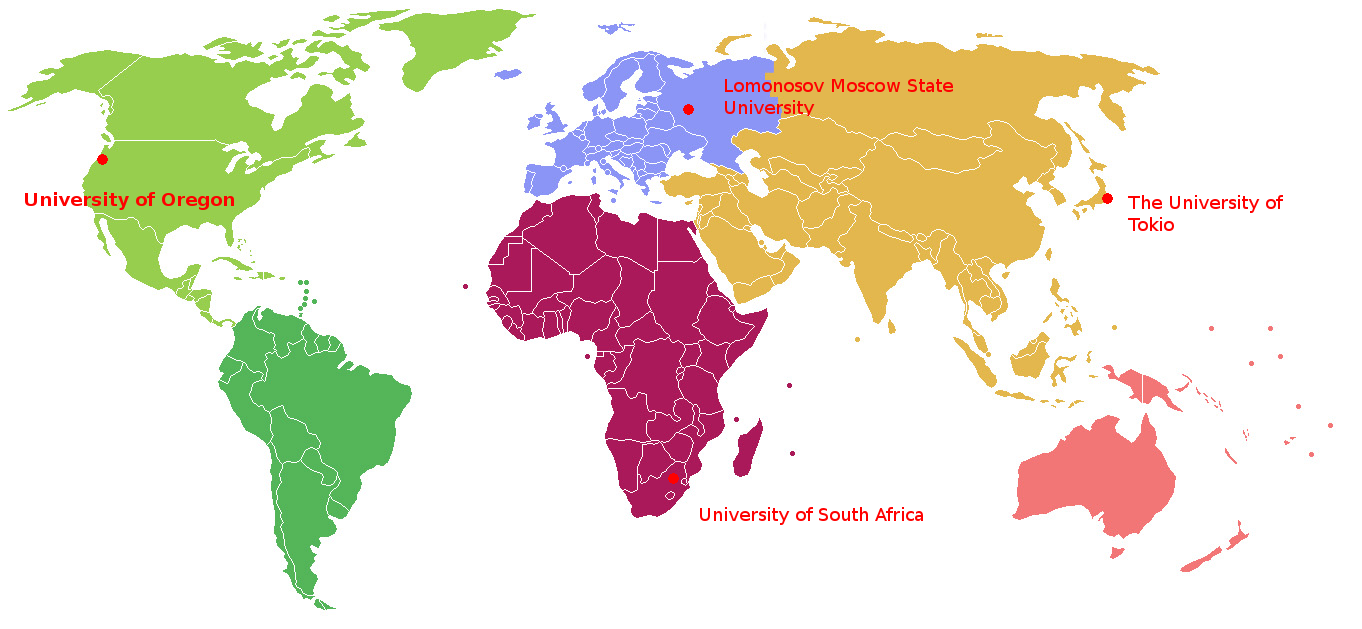
\includegraphics[scale = 0.3]{imagenes/mapa.png}
  \caption{Ubicación de las universidades elegidas}
  \label{histogramaprobabilidadesModel1}
\end{figure}


Los experimentos se realizaron sobre en una computadora conectada a internet (proveedor Fibertel) por medio de un enlace WiFi. Se utilizaron los siguientes comandos (donde n es el tamaño de la ráfaga) 
\begin{itemize}
  \item EEUU:      sudo python traceroute.py www.cs.uoregon.edu -tr n -p 0.3 -m 30 -o EEUU\_OREGON\_n
  \item JAPON:     sudo python traceroute.py www.u-tokyo.ac.jp  -tr n -p 0.3 -m 30 -o JAP\_n
  \item RUSIA:     sudo python traceroute.py msu.ru             -tr n -p 0.3 -m 30 -o RUSIA\_n
  \item SUDAFRICA: sudo python traceroute.py www.unisa.ac.za    -tr n -p 0.3 -m 30 -o AFR\_n 
\end{itemize}

Los resultados obtenidos son los siguientes.

\begin{figure}[H]
  \centering
  %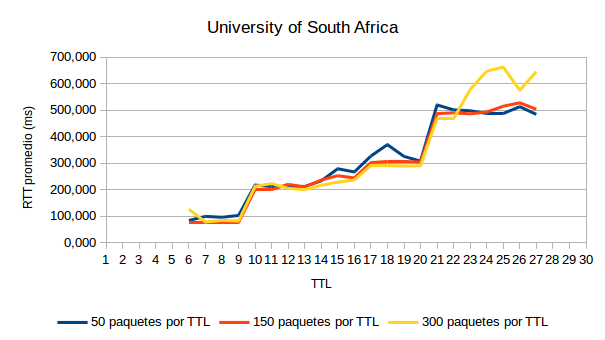
\includegraphics[scale = 0.8]{imagenes/africaTTL.png}
  \caption{RTT estimado del traceroute a la Universidad de Sudafrica}
  \label{africaTTL}
  
  \subfigure[RTT promedio por TTL]{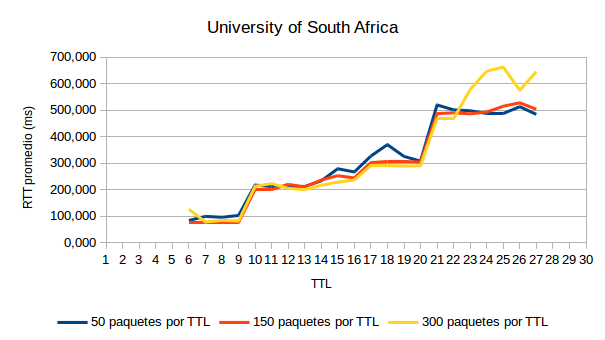
\includegraphics[scale = 0.8]{imagenes/africaTTL.png} }
  \subfigure[RTT relativos entre saltos]{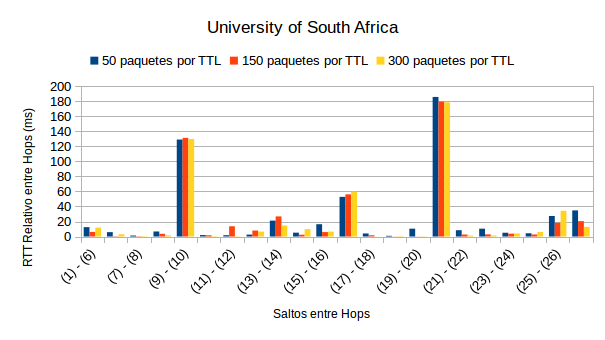
\includegraphics[scale = 0.8]{imagenes/africaRTTrelativos.png}}
\end{figure}

\begin{figure}[H]
  \centering
  %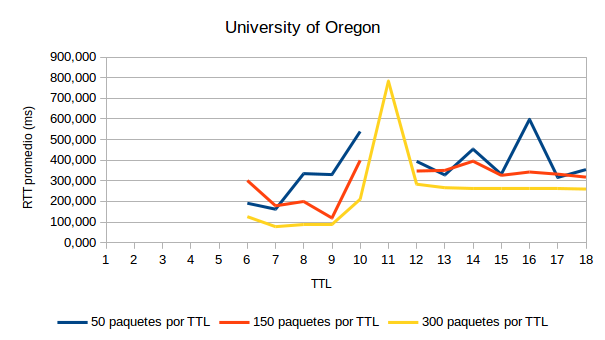
\includegraphics[scale = 0.8]{imagenes/eeuuTTL.png}
  \caption{RTT estimado del traceroute a la Universidad de Oregón }
  \label{eeuuTTL}
  \subfigure[RTT promedio por TTL]{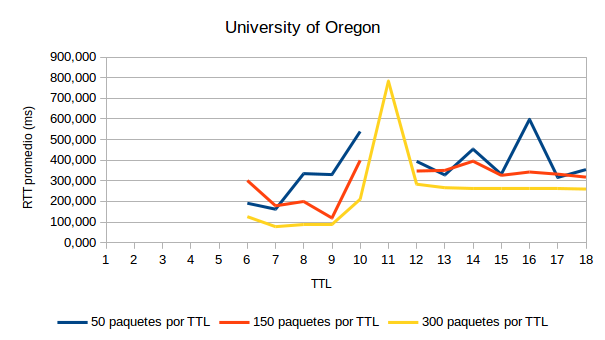
\includegraphics[scale = 0.8]{imagenes/eeuuTTL.png} }
  \subfigure[RTT relativos entre saltos]{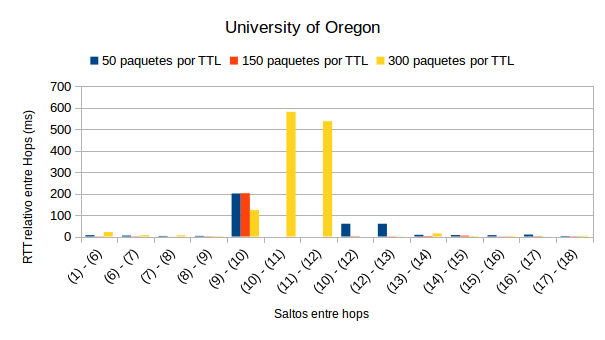
\includegraphics[scale = 0.8]{imagenes/eeuuRTTrelativos.png}}
\end{figure}
\begin{figure}[H]
  \centering
  %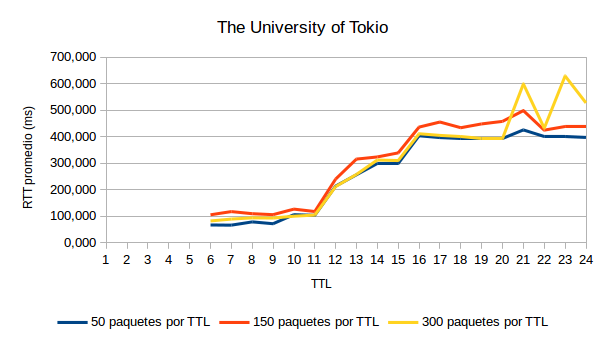
\includegraphics[scale = 0.8]{imagenes/japonTTL.png}
  \caption{RTT promedio de traceroute a la Universidad de Tokio }
  \label{japonTTL}
  \subfigure[RTT promedio por TTL]{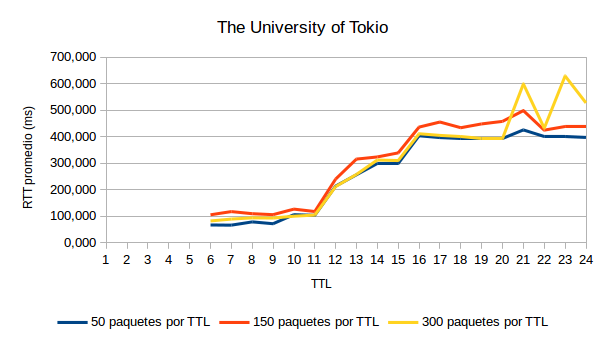
\includegraphics[scale = 0.8]{imagenes/japonTTL.png} }
  \subfigure[RTT relativos entre saltos]{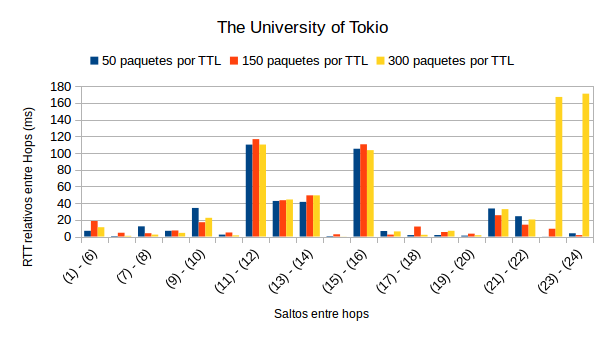
\includegraphics[scale = 0.8]{imagenes/japonRTTrelativos.png}}
  
\end{figure}
\begin{figure}[H]
  \centering
  %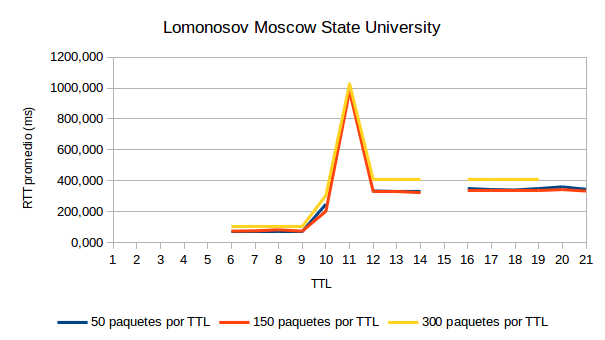
\includegraphics[scale = 0.8]{imagenes/rusiaTTL.png}
  \caption{RTT promedio del traceroute a la Universidad de Moscú}
  \label{rusiaTTL}
  \subfigure[RTT promedio por TTL]{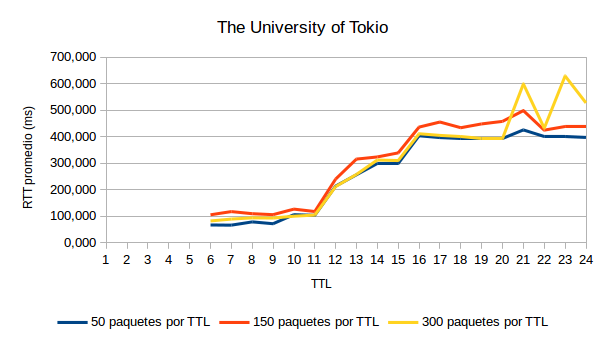
\includegraphics[scale = 0.8]{imagenes/japonTTL.png} }
  \subfigure[RTT relativos entre saltos]{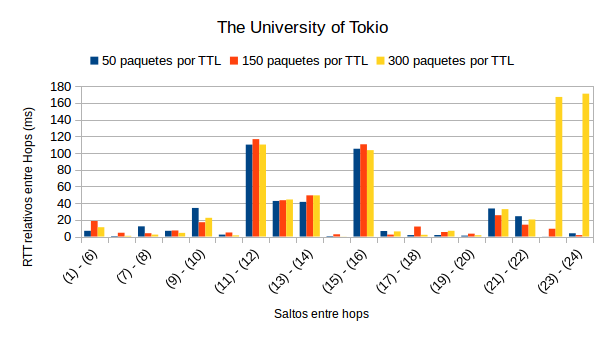
\includegraphics[scale = 0.8]{imagenes/japonRTTrelativos.png}}
  
\end{figure}

\begin{table}[]
\centering
\caption{Africa}
%\label{Universidad}
\begin{tabular}{ | c | c | c | c | c | c | }
	\hline 
  & & & Rafaga = 50 & Rafaga = 150 &Rafaga = 300  \\ %\hline
  TTL	&         IP        & 	        Pais      &  	 RTT Filtrado Prom  &	 RTT Filtrado Prom  & RTT Filtrado Prom  \\ \hline  
  1	&192.168.0.1        & 	       Local      &  	      63.183 ms     &	       63.66 ms     &      60.306 ms     \\ \hline  
  2	&None               & 	      Unknown     &  	      Unknown       &	      Unknown       &      Unknown       \\ \hline  
  3	&None               & 	      Unknown     &  	      Unknown       &	      Unknown       &      Unknown       \\ \hline  
  4	&None               & 	      Unknown     &  	      Unknown       &	      Unknown       &      Unknown       \\ \hline  
  5	&None               & 	      Unknown     &  	      Unknown       &	      Unknown       &      Unknown       \\ \hline  
  6	&200.89.164.129     & 	     Argentina    &  	      75.735 ms     &	      69.777 ms     &      72.186 ms     \\ \hline  
  7	&200.89.165.130     & 	     Argentina    &  	        81.6 ms     &	      69.322 ms     &      75.228 ms     \\ \hline  
  8	&200.89.165.222     & 	     Argentina    &  	      82.939 ms     &	      69.796 ms     &      74.685 ms     \\ \hline  
  9	&195.22.220.172     & 	       Italy      &  	      72.147 ms     &	       66.17 ms     &      72.982 ms     \\ \hline  
  10	&89.221.41.161      & 	       Italy      &  	     201.218 ms     &	     197.541 ms     &     202.749 ms     \\ \hline  
  11	&89.221.41.161      & 	       Italy      &  	     199.258 ms     &	      195.86 ms     &     203.352 ms     \\ \hline  
  12	&154.54.9.17        & 	   United States  &  	     201.047 ms     &	     209.585 ms     &     203.779 ms     \\ \hline  
  13	&154.54.24.233      & 	   United States  &  	     198.495 ms     &	     201.588 ms     &      197.17 ms     \\ \hline  
  14	&154.54.24.197      & 	   United States  &  	     219.718 ms     &	     228.412 ms     &     211.934 ms     \\ \hline  
  15	&154.54.24.221      & 	   United States  &  	     224.876 ms     &	       225.9 ms     &     221.758 ms     \\ \hline  
  16	&154.54.40.109      & 	   United States  &  	     241.303 ms     &	     231.854 ms     &     228.356 ms     \\ \hline  
  17	&154.54.42.86       & 	   United States  &  	     294.135 ms     &	     288.052 ms     &     287.978 ms     \\ \hline  
  18	&154.54.58.186      & 	   United States  &  	     298.166 ms     &	     289.808 ms     &     287.868 ms     \\ \hline  
  19	&154.54.56.238      & 	   United States  &  	     297.178 ms     &	     289.593 ms     &     287.225 ms     \\ \hline  
  20	&149.14.80.210      & 	   United States  &  	      286.71 ms     &	     289.823 ms     &     287.583 ms     \\ \hline  
  21	&196.32.209.174     & 	    South Africa  &  	     472.497 ms     &	      469.31 ms     &     466.299 ms     \\ \hline  
  22	&155.232.6.65       & 	    South Africa  &  	      480.99 ms     &	     471.961 ms     &      467.52 ms     \\ \hline  
  23	&155.232.6.37       & 	    South Africa  &  	     470.571 ms     &	     469.022 ms     &     465.979 ms     \\ \hline  
  24	&155.232.6.33       & 	    South Africa  &  	      475.67 ms     &	     472.859 ms     &     470.095 ms     \\ \hline  
  25	&155.232.6.142      & 	    South Africa  &  	     471.279 ms     &	     475.578 ms     &     464.099 ms     \\ \hline  
  26	&155.232.6.145      & 	    South Africa  &  	     498.626 ms     &	     493.943 ms     &     498.355 ms     \\ \hline  
  27	&155.232.6.138      & 	    South Africa  &  	     463.824 ms     &	     473.392 ms     &     511.219 ms     \\ \hline  
  28	&None               & 	      Unknown     &  	      Unknown       &	      Unknown       &      Unknown       \\ \hline  
  29	&None               & 	      Unknown     &  	      Unknown       &	      Unknown       &      Unknown       \\ \hline  
  30	&None               & 	      Unknown     &  	      Unknown       &	      Unknown       &      Unknown       \\ \hline  
\end{tabular}
\end{table}


\begin{table}[]
\centering
\caption{EEUU}
%\label{Universidad}
\begin{tabular}{ | c | c | c | c | c | c | }
	\hline 
  & & & 50	& 150	& 300 \\ %\hline
TTL	&          IP         	     &    Pais        & 	 RTT Filtrado Prom  	&  RTT Filtrado Prom  & 	 RTT Filtrado Prom  \\ \hline  
1	& 192.168.0.1       &   	       Local      &   	       99.53 ms    &  	     103.514 ms   &   	      57.461 ms   \\ \hline    
2	& None               &  	      Unknown     &   	      Unknown      &  	      Unknown     &   	      Unknown     \\ \hline    
3	& None               &  	      Unknown     &   	      Unknown      &  	      Unknown     &   	      Unknown     \\ \hline    
4	& None               &  	      Unknown     &   	      Unknown      &  	      Unknown     &   	      Unknown     \\ \hline    
5	& None               &  	      Unknown     &   	      Unknown      &  	      Unknown     &   	      Unknown     \\ \hline    
6	& 200.89.165.141    &   	     Argentina    &   	     106.059 ms    &  	     102.341 ms   &   	      78.394 ms   \\ \hline    
7	& 200.89.165.130    &   	     Argentina    &   	     101.341 ms    &  	     103.905 ms   &   	      71.902 ms   \\ \hline    
8	& 200.89.165.222    &   	     Argentina    &   	     104.182 ms    &  	     103.432 ms   &   	      77.629 ms   \\ \hline    
9	& 190.216.88.33     &   	     Argentina    &   	     107.429 ms    &  	     101.819 ms   &   	      79.446 ms   \\ \hline    
10	& 67.17.94.249     &    	   United States  &   	     308.066 ms    &  	     303.806 ms   &   	     202.742 ms   \\ \hline    
11	& None               &  	      Unknown     &   	      Unknown      &  	      Unknown     &   	     783.798 ms   \\ \hline    
12	& 4.69.132.149    &     	   United States  &   	     367.776 ms    &  	     305.802 ms   &   	     246.129 ms   \\ \hline    
13	& 4.69.132.149    &     	   United States  &   	     307.944 ms    &  	     307.181 ms   &   	     247.065 ms   \\ \hline    
14	& 4.53.200.2      &     	   United States  &   	     299.937 ms    &  	     309.681 ms   &   	     261.722 ms   \\ \hline    
15	& 207.98.64.165     &   	   United States  &   	     306.661 ms    &  	     305.197 ms   &   	     258.771 ms   \\ \hline    
16	& 207.98.68.182     &   	   United States  &   	     313.137 ms    &  	     306.078 ms   &   	     261.577 ms   \\ \hline    
17	& 128.223.2.1       &   	   United States  &   	     303.678 ms    &  	     308.079 ms   &   	     261.194 ms   \\ \hline    
18	& 128.223.4.25      &   	   United States  &   	     306.301 ms    &  	     306.542 ms   &   	      257.81 ms   \\ \hline    
\end{tabular}
\end{table}


\begin{table}[]
\centering
\caption{Japón}
%\label{Universidad}
\begin{tabular}{ | c | c | c | c | c | c | }
\hline
 &&& 50 & 150 & 300 \\ %\hline
TTL	&         IP     &    	        Pais     &   	 RTT Filtrado Prom & 	 RTT Filtrado Prom  &	 RTT Filtrado Prom \\ \hline  
1	&192.168.0.1     &    	       Local     &   	      59.684 ms    & 	       62.26 ms     &	      65.531 ms  \\ \hline    
2	&None            &    	      Unknown    &   	      Unknown      & 	      Unknown       &	      Unknown    \\ \hline    
3	&None            &    	      Unknown    &   	      Unknown      & 	      Unknown       &	      Unknown    \\ \hline    
4	&None            &    	      Unknown    &   	      Unknown      & 	      Unknown       &	      Unknown    \\ \hline    
5	&None            &    	      Unknown    &   	      Unknown      & 	      Unknown       &	      Unknown    \\ \hline    
6	&200.89.164.129  &    	     Argentina   &   	      66.602 ms    & 	      80.867 ms     &	      76.751 ms  \\ \hline    
7	&200.89.165.5    &    	     Argentina   &   	      65.983 ms    & 	      85.396 ms     &	      77.617 ms  \\ \hline    
8	&200.89.165.250  &    	     Argentina   &   	      78.198 ms    & 	      81.414 ms     &	      79.964 ms  \\ \hline    
9	&185.70.203.56   &    	       Italy     &   	      71.299 ms    & 	      88.681 ms     &	      75.557 ms  \\ \hline    
10	&195.22.219.3    &    	       Italy     &   	     105.539 ms    & 	      105.86 ms     &	      98.037 ms  \\ \hline    
11	&195.22.219.3    &    	       Italy     &   	       103.2 ms    & 	     100.989 ms     &	      99.468 ms  \\ \hline    
12	&149.3.181.65    &    	       Italy     &   	     213.327 ms    & 	     217.664 ms     &	     209.684 ms  \\ \hline    
13	&129.250.2.227   &    	   United States &   	      255.97 ms    & 	     261.183 ms     &	     254.077 ms  \\ \hline    
14	&129.250.4.13    &    	   United States &   	     297.467 ms    & 	     310.539 ms     &	     303.424 ms  \\ \hline    
15	&129.250.2.54    &    	   United States &   	     298.115 ms    & 	     307.844 ms     &	     303.238 ms  \\ \hline    
16	&129.250.3.86    &    	   United States &   	     403.231 ms    & 	     418.358 ms     &	     406.681 ms  \\ \hline    
17	&129.250.6.188   &    	   United States &   	     396.553 ms    & 	     416.043 ms     &	     400.489 ms  \\ \hline    
18	&129.250.2.255   &    	   United States &   	     394.784 ms    & 	     404.056 ms     &	     398.441 ms  \\ \hline    
19	&61.200.80.218   &    	       Japan     &   	     392.899 ms    & 	     409.514 ms     &	      391.58 ms  \\ \hline    
20	&158205192173	 &      Japan        	  &   391.804 ms     	    & 412.988 ms     	     &393.182 ms     \\ \hline    
21	&158.205.192.86  &    	       Japan     &   	     425.468 ms    & 	     438.572 ms     &	     426.033 ms  \\ \hline     
22	&158205121250	 &      Japan        	  &   401.164 ms     	    &  424.37 ms     	     &405.547 ms     \\ \hline    
23	&154.34.240.254  &    	       Japan     &   	     400.949 ms    & 	     415.033 ms     &	       572.7 ms  \\ \hline    
24	&210152135178	 &      Japan        	  &    397.01 ms     	    & 416.837 ms     	     &401.609 ms         \\ \hline

\end{tabular}
\end{table}

\begin{table}[]
\centering
\caption{Rusia}
%\label{Universidad}
\begin{tabular}{ | c | c | c | c | c | c | }
\hline
 & & & 50 & 150 & 300 \\ %\hline
TTL	&         IP    &     	        Pais     &   	 RTT Filtrado Prom&  	 RTT Filtrado Prom&  	 RTT Filtrado Prom  \\ \hline
1	&192.168.0.1    &     	       Local     &   	      66.082 ms   &  	     101.009 ms   &  	      62.141 ms \\ \hline    
2	&None           &     	      Unknown    &   	      Unknown     &  	      Unknown     &  	      Unknown   \\ \hline    
3	&None           &     	      Unknown    &   	      Unknown     &  	      Unknown     &  	      Unknown   \\ \hline    
4	&None           &     	      Unknown    &   	      Unknown     &  	      Unknown     &  	      Unknown   \\ \hline    
5	&None           &     	      Unknown    &   	      Unknown     &  	      Unknown     &  	      Unknown   \\ \hline    
6	&200.89.164.141 &     	     Argentina   &   	      67.789 ms   &  	     103.426 ms   &  	      74.055 ms \\ \hline    
7	&200.89.165.130 &     	     Argentina   &   	       63.79 ms   &  	     101.435 ms   &  	      76.409 ms \\ \hline    
8	&200.89.165.222 &     	     Argentina   &   	      64.843 ms   &  	     103.571 ms   &  	       83.03 ms \\ \hline    
9	&190.216.88.33  &     	     Argentina   &   	      68.088 ms   &  	     101.673 ms   &  	      73.911 ms \\ \hline    
10	&67.17.99.233   &     	   United States &   	     237.063 ms   &  	     306.126 ms   &  	     203.308 ms \\ \hline    
11	&None           &     	      Unknown    &   	      Unknown     &  	    1027.876 ms   &  	     980.007 ms \\ \hline    
12	&4.69.158.253   &     	   United States &   	      326.02 ms   &  	     407.603 ms   &  	     327.569 ms \\ \hline    
13	&4.69.158.253   &     	   United States &   	     325.194 ms   &  	     408.104 ms   &  	      327.74 ms \\ \hline    
14	&213242110198	  & United Kingdom   	    & 325.508 ms     	     &408.248 ms     	     &323.149 ms     \\ \hline
15	&None           &     	      Unknown    &   	      Unknown     &  	      Unknown     &  	      Unknown   \\ \hline    
16	&194.85.40.229  &     	       Russia    &   	      338.62 ms   &  	     410.191 ms   &  	     336.288 ms \\ \hline    
17	&194190254118	  &     Russia       	    & 336.555 ms     	     &410.227 ms     	     &335.396 ms     \\ \hline
18	&93.180.0.172   &     	       Russia    &   	     339.032 ms   &  	     409.307 ms   &  	     335.718 ms \\ \hline    
19	&188.44.33.30   &     	       Russia    &   	     341.636 ms   &  	     409.164 ms   &  	     337.758 ms \\ \hline    
20	&188.44.33.2    &     	       Russia    &   	     346.137 ms   &  	      408.97 ms   &  	     343.093 ms \\ \hline    
21	&188.44.50.103  &     	       Russia    &   	     340.466 ms   &  	     410.042 ms   &  	     333.481 ms \\ \hline     

\end{tabular}
\end{table}
	
	Para cada experimento:
		Mapa con los puntos marcados
		Grafico de RTT (lineas)
		Grafico de RTT relativos (barras)
		Tabla de saltos (agregar ips)

		
		
%%%%%%%%%%%%%%%%%%%%%%%%%%%%%%%%%%%%%%%%%%%%%%%%%%%%%%%%%%%%%%%%%%%%
\subsection{Segunda consigna: gráficos y análisis}


Realizaremos un análisis que permitará detectar los saltos correspondientes a enlaces intercontinentales. Para esto usaremos 

Para obtener los datos de los experimentos, consideramos lo siguiente:
Para calcular el RTT para un determinado Hop(salto) utilizamos un promedio de las muestras particulares para cada universidad.
Para usar el metodo de calculo de outlier, tomamos como hipotesis que los RTT relativos (entre hops) cuanto mas grande sean, mayor es la posibilidad de ser un salto intercontinental. Partiendo de esta base, llamamos al metodo de cimbala con el set de datos de RTT relativos.

\subsubsection{Experimentos}
\textbf{The university of tokio} \\

\textbf{Ruta de IPs:} \{ [192.168.10.1]; [200.89.160.17]; [200.89.165.222];
 [195.22.220.64]; [195.22.219.17]; [195.22.219.17]; [149.3.181.65]; [129.250.2.227]
 [129.250.4.13]; [129.250.2.54]; [129.250.3.86]; [129.250.6.188]; [129.250.2.255];
 [61.200.80.218]; [158.205.192.173]; [158.205.192.86]; [158.205.121.250];
 [154.34.240.254]; [210.152.135.178]\}

En el primer gráfico mostramos como incrementa el RTT a medida que se van enviando los paquetes con un TTL determinado. Se puede ver que cuando enviamos los paquetes con TTLs 2,3, y 4 no obtenemos respuesta, suponemos que hay servidores a dicha distancia no estan configurados para responder paquetes ICMP de tipo Echo Request,o que se perdieron en la red. Tambien, como habiamos dicho antes, suponemos que los saltos de incremento del RTT se debe a una conexión intercontinetal, asi que podemos asumir que hay posible conexiones ente los Hops 1-2, 9-10, 13-14 y 15-16.
Para comprobar esta hipotesis, tomamos el RTT relativo entre Hops y se los pasamos al metodo de cimbala y nos da como resultado que los posibles candidatos son:
(9, 5, 7, 11)


\begin{center}
   \begin{tabular}{ |l | c | r | }
     \hline
     \textbf{Origen} & \textbf{Destino} & \textbf{RRT relativo (ms)} \\ \hline
     Home & Argentina & 20.868 \\ \hline
     Argentina & Argentina & 0.162 \\ \hline
     Argentina & Italy & 3.043 \\ \hline
     Italy & Italy & 30.260 \\ \hline
     Italy & Italy & 8.189 \\ \hline
     Italy & Italy & 109.476\\ \hline
     Italy & United States & 1.993\\ \hline
     United States & United States & 52.135 \\ \hline
     United States & United States & 0.485\\ \hline
     United States & United States & 111.830\\ \hline
     United States & United States & 1.617 \\ \hline
     United States & United States & 48.441 \\ \hline
     United States & Japan & 32.720 \\ \hline
     Japan & Japan & 10.492 \\ \hline
     Japan & Japan & 4.534 \\ \hline
     Japan & Japan & 26.721 \\ \hline
     Japan & Japan & 7.028 \\ \hline
     Japan & Japan & 19.043 \\ \hline
   \end{tabular}
 \end{center}
